%%%%%%%%%%%%%%%%%%%%%%%%%%%%%%%%%%%%%%%%%
% Masters/Doctoral Thesis 
% LaTeX Template
% Version 2.2.2 (20/2/16)
%
% This template has been downloaded from:
% http://www.LaTeXTemplates.com
%
% Version 2.x major modifications by:
% Vel (vel@latextemplates.com)
%
% This template is based on a template by:
% Steve Gunn (http://users.ecs.soton.ac.uk/srg/softwaretools/document/templates/)
% Sunil Patel (http://www.sunilpatel.co.uk/thesis-template/)
%
% Template license:
% CC BY-NC-SA 3.0 (http://creativecommons.org/licenses/by-nc-sa/3.0/)
%
%%%%%%%%%%%%%%%%%%%%%%%%%%%%%%%%%%%%%%%%%

%----------------------------------------------------------------------------------------
%	PACKAGES AND OTHER DOCUMENT CONFIGURATIONS
%----------------------------------------------------------------------------------------

\newenvironment{dedication}
  {\clearpage           % we want a new page
   \thispagestyle{empty}% no header and footer
   \vspace*{\stretch{1}}% some space at the top 
   \itshape             % the text is in italics  
   \raggedleft          % flush to the right margin
  }
  {\par % end the paragraph
   \vspace{\stretch{3}} % space at bottom is three times that at the top
   \clearpage           % finish off the page
  }
  
\newcommand*\justify{%
  \fontdimen2\font=0.4em% interword space
  \fontdimen3\font=0.2em% interword stretch
  \fontdimen4\font=0.1em% interword shrink
  \fontdimen7\font=0.1em% extra space
  \hyphenchar\font=`\-% allowing hyphenation
}

\documentclass[
oneside,
11pt, % The default document font size, options: 10pt, 11pt, 12pt
%oneside, % Two side (alternating margins) for binding by default, uncomment to switch to one side
english, % ngerman for German
onehalfspacing, % Single line spacing, alternatives: onehalfspacing or doublespacing
%draft, % Uncomment to enable draft mode (no pictures, no links, overfull hboxes indicated)
%nolistspacing, % If the document is onehalfspacing or doublespacing, uncomment this to set spacing in lists to single
%liststotoc, % Uncomment to add the list of figures/tables/etc to the table of contents
%toctotoc, % Uncomment to add the main table of contents to the table of contents
%parskip, % Uncomment to add space between paragraphs
%nohyperref, % Uncomment to not load the hyperref package
headsepline, % Uncomment to get a line under the header
]{MastersDoctoralThesis} % The class file specifying the document structure

\usepackage[utf8]{inputenc} % Required for inputting international characters
\usepackage[T1]{fontenc} % Output font encoding for international characters 

\usepackage{palatino} % Use the Palatino font by default

\usepackage[backend=bibtex,style=authoryear,natbib=true]{biblatex} % Use the bibtex backend with the authoryear citation style (which resembles APA)

\addbibresource{references.bib} % The filename of the bibliography

\usepackage[autostyle=true]{csquotes} % Required to generate language-dependent quotes in the bibliography

% Additional packages
\usepackage[dvipsnames]{xcolor}
\usepackage{todonotes}
\usepackage{listings}
\usepackage{soul}
\usepackage{rotating}
\usepackage{tikz}
\usetikzlibrary{shapes,arrows,snakes}
\usepackage{courier}
\usepackage{graphicx}
\usepackage{float}
\usepackage{microtype}
\usepackage{pdfpages}
\usepackage{lineno}

\lstset{basicstyle=\ttfamily,breaklines=true}

%----------------------------------------------------------------------------------------
%	MARGIN SETTINGS
%----------------------------------------------------------------------------------------

\geometry{
	paper=a4paper, % Change to letterpaper for US letter
	inner=2.5cm, % Inner margin
	outer=3.8cm, % Outer margin
	bindingoffset=2cm, % Binding offset
	top=1.5cm, % Top margin
	bottom=1.5cm, % Bottom margin
	%showframe,% show how the type block is set on the page
}

%----------------------------------------------------------------------------------------
%	THESIS INFORMATION
%----------------------------------------------------------------------------------------

\thesistitle{Generating Article Placeholders from Wikidata for Wikipedia:\\Increasing Access to Free and Open Knowledge} % Your thesis title, this is used in the title and abstract, print it elsewhere with \ttitle
\supervisor{Prof. Dr. Debora \textsc{Weber-Wulff}} % Your supervisor's name, this is used in the title page, print it elsewhere with \supname
\examiner{Lydia \textsc{Pintscher}} % Your examiner's name, this is not currently used anywhere in the template, print it elsewhere with \examname
\degree{Bachelor of Science} % Your degree name, this is used in the title page and abstract, print it elsewhere with \degreename
\author{Lucie-Aim\'{e}e \textsc{Kaffee}} % Your name, this is used in the title page and abstract, print it elsewhere with \authorname
\addresses{} % Your address, this is not currently used anywhere in the template, print it elsewhere with \addressname

\subject{Computer Science} % Your subject area, this is not currently used anywhere in the template, print it elsewhere with \subjectname
\keywords{} % Keywords for your thesis, this is not currently used anywhere in the template, print it elsewhere with \keywordnames
\university{\href{https://www.htw-berlin.de/}{HTW Berlin -- University of Applied Sciences}} % Your university's name and URL, this is used in the title page and abstract, print it elsewhere with \univname
\department{\href{http://www.f4.htw-berlin.de/}{International Media and Computing}} % Your department's name and URL, this is used in the title page and abstract, print it elsewhere with \deptname
\group{\href{}{}} % Your research group's name and URL, this is used in the title page, print it elsewhere with \groupname
\faculty{\href{http://faculty.university.com}{Faculty IV}} % Your faculty's name and URL, this is used in the title page and abstract, print it elsewhere with \facname

\hypersetup{pdftitle=\ttitle} % Set the PDF's title to your title
\hypersetup{pdfauthor=\authorname} % Set the PDF's author to your name
\hypersetup{pdfkeywords=\keywordnames} % Set the PDF's keywords to your keywords

\begin{document}

\frontmatter % Use roman page numbering style (i, ii, iii, iv...) for the pre-content pages

\pagestyle{plain} % Default to the plain heading style until the thesis style is called for the body content

%----------------------------------------------------------------------------------------
%	TITLE PAGE
%----------------------------------------------------------------------------------------

\begin{titlepage}
\begin{center}

{\scshape\LARGE \textcolor{magenta}{HTW Berlin \\ University of Applied Sciences}\par}\vspace{2cm} % University name
%\textsc{\Large Doctoral Thesis}\\[0.5cm] % Thesis type

\HRule \\[0.4cm] % Horizontal line
{\huge \bfseries \ttitle\par}\vspace{0.4cm} % Thesis title
\HRule \\[1.5cm] % Horizontal line
 
\begin{minipage}[t]{0.4\textwidth}
\begin{flushleft} \large
\emph{Author:}\\
\textcolor{magenta}{\authorname} % Author name - remove the \href bracket to remove the link
\end{flushleft}
\end{minipage}
\begin{minipage}[t]{0.4\textwidth}
\begin{flushright} \large
\emph{First Examiner:} \\
\href{http://people.f4.htw-berlin.de/~weberwu/}{\supname}\\
\emph{Second Examiner:} \\
\href{https://about.me/lydia.pintscher}{\examname} % Supervisor name - remove the \href bracket to remove the link  
\end{flushright}
\end{minipage}\\[3cm]
 
\large \textit{A thesis submitted in fulfillment of the requirements\\ for the degree of \degreename}\\[1.7cm] % University requirement text
%\textit{in the}\\[0.4cm]
%\groupname\\
\deptname\\\facname\\[2cm] % Research group name and department name

 
{\large \today}\\[4cm] % Date
%\includegraphics{Logo} % University/department logo - uncomment to place it
 
\vfill
\end{center}
\end{titlepage}

%----------------------------------------------------------------------------------------
%	DECLARATION PAGE
%----------------------------------------------------------------------------------------

\begin{declaration}
\addchaptertocentry{\authorshipname}

\noindent I, \authorname, declare that this thesis titled, \enquote{\ttitle} and the work presented in it are my own. I confirm that:

\begin{itemize} 
\item This work was done wholly or mainly while in candidature for a research degree at this University.
\item Where any part of this thesis has previously been submitted for a degree or any other qualification at this University or any other institution, this has been clearly stated.
\item Where I have consulted the published work of others, this is always clearly attributed.
\item Where I have quoted from the work of others, the source is always given. With the exception of such quotations, this thesis is entirely my own work.
\item I have acknowledged all main sources of help.
\item Where the thesis is based on work done by myself jointly with others, I have made clear exactly what was done by others and what I have contributed myself.\\
\end{itemize}
 
\noindent Signed:\\
\rule[0.5em]{25em}{0.5pt} % This prints a line for the signature
 
\noindent Date:\\
\rule[0.5em]{25em}{0.5pt} % This prints a line to write the date
\end{declaration}

\cleardoublepage

%----------------------------------------------------------------------------------------
%	CC-BY-SA PAGE
%----------------------------------------------------------------------------------------
\clearpage\null\vfill
\pagestyle{empty}
\begin{minipage}[b]{0.9\textwidth}
\footnotesize\raggedright
\setlength{\parskip}{0.5\baselineskip}
\copyright 2016 by \authorname. \\
\textit{Generating Article Placeholders from Wikidata for Wikipedia: Increasing Access to Free and Open Knowledge} is made available under the Creative Commons Attribution-ShareAlike 4.0 International License. To view a copy of this license, visit \url{http://creativecommons.org/licenses/by-sa/4.0/}.
\end{minipage}
\vspace*{2\baselineskip}
\cleardoublepage

%----------------------------------------------------------------------------------------
%	DEDICATION PAGE
%----------------------------------------------------------------------------------------

%\vspace*{0.2\textheight}
\begin{dedication}
 To Amaru and Laura \\
 And my parents
\end{dedication}

%----------------------------------------------------------------------------------------
%	ABSTRACT PAGE
%----------------------------------------------------------------------------------------

\begin{abstract}
\addchaptertocentry{\abstractname} % Add the abstract to the table of contents

The Thesis Abstract is written here (and usually kept to just this page). The page is kept centered vertically so can expand into the blank space above the title too\ldots

\end{abstract}

%----------------------------------------------------------------------------------------
%	ACKNOWLEDGEMENTS
%----------------------------------------------------------------------------------------

\begin{acknowledgements}
\addchaptertocentry{\acknowledgementname} % Add the acknowledgements to the table of contents

I would like to thank my supervisor, Prof. Dr. Weber-Wulff, for her guidance throughout 

\end{acknowledgements}

%----------------------------------------------------------------------------------------
%	Disclaimer
%----------------------------------------------------------------------------------------

 \begin{centering}
\chapter*{Disclaimer}

This thesis was written in cooperation with \textbf{Wikimedia Deutschland}. \\
The views expressed in this thesis are those of the student and do not necessarily express the views of \textbf{Wikimedia Deutschland} or the \textbf{Hochschule für Technik und Wirtschaft Berlin}. \\
The source code written as part of the thesis is published under GNU General Public License 2.0 and is in active development. Even though it was developed by the student, the Wikidata team at Wikimedia Deutschland contributed to it with input and code review.

\end{centering}


%----------------------------------------------------------------------------------------
%	LIST OF CONTENTS/FIGURES/TABLES PAGES
%----------------------------------------------------------------------------------------

\tableofcontents % Prints the main table of contents

\listoffigures % Prints the list of figures

%\listoftables % Prints the list of tables

%----------------------------------------------------------------------------------------
%	ABBREVIATIONS
%----------------------------------------------------------------------------------------

% \begin{abbreviations}{ll} % Include a list of abbreviations (a table of two columns)
% 
% \textbf{LAH} & \textbf{L}ist \textbf{A}bbreviations \textbf{H}ere\\
% \textbf{WSF} & \textbf{W}hat (it) \textbf{S}tands \textbf{F}or\\
% 
% \end{abbreviations}

%----------------------------------------------------------------------------------------
%	PHYSICAL CONSTANTS/OTHER DEFINITIONS
%----------------------------------------------------------------------------------------

% \begin{constants}{lr@{${}={}$}l} % The list of physical constants is a three column table
% 
% % The \SI{}{} command is provided by the siunitx package, see its documentation for instructions on how to use it
% 
% 	Speed of Light & $c_{0}$ & \SI{2.99792458e8}{\meter\per\second} (exact)\\
% %Constant Name & $Symbol$ & $Constant Value$ with units\\
% 
% \end{constants}

%----------------------------------------------------------------------------------------
%	SYMBOLS
%----------------------------------------------------------------------------------------

% \begin{symbols}{lll} % Include a list of Symbols (a three column table)
% 
% $a$ & distance & \si{\meter} \\
% $P$ & power & \si{\watt} (\si{\joule\per\second}) \\
% %Symbol & Name & Unit \\
% 
% \addlinespace % Gap to separate the Roman symbols from the Greek
% 
% $\omega$ & angular frequency & \si{\radian} \\
% 
% \end{symbols}

%----------------------------------------------------------------------------------------
%	THESIS CONTENT - CHAPTERS
%----------------------------------------------------------------------------------------

\mainmatter % Begin numeric (1,2,3...) page numbering

\pagestyle{thesis} % Return the page headers back to the "thesis" style

\chapter{Introduction}

One of the greatest barriers for accessing knowledge on the Internet is language. The tendency is to provide information in one or at most a few languages, which makes it hard for speakers of all other languages to access that same information. This is also an issue with Wikipedia, a project used all across the globe by all kinds of people. There are many topics that are only covered in a few languages on Wikipedia. People who do not speak these languages do not have access to all the information available and potentially vital to them. This is an important issue that needs to be addressed. \\

To close this informational gap, the ArticlePlaceholder extension was developed. The aim is to give more people more access to more knowledge by making use of Wikipedia’s reach and Wikidata’s multilingual data. \todo{Short intro to Wikidata}\\
ArticlePlaceholder generates content pages on Wikipedia in the community's language from data and offer the possibility to create actual articles and translate them. It aims to support readers as well as editors. \\
\\
In the course of this thesis, an introduction to the fundamentals needed for the project will be given as well as an overview over the previous work done with regards to Wikidata and Wikipedia. \\
Since a lot of the development was user-centric, personas were created to develop scenarios and user stories. From those scenarios non-functional and functional requirements were derived. The implementation realizes many of the requirements and includes the technical aspects of the extension.

\todo{delete}\st{In the course of this thesis, there will be an introduction to the fundamentals needed for the project, an overview of the previous work done with regards to Wikidata and Wikipedia, the requirements that should be fulfilled for the project, and the implementation of the technical aspects of the extension.} 
\subsection{Wikipedia}
Wikipedia is one of the largest websites in the world with articles in over 250 languages. As of January 2016, the English Wikipedia alone amounts to 5,000,000 articles. 
The concept of Wikipedia is fairly simple: An open encyclopaedia anyone can edit. It was launched on January 15, 2001. 

\begin{itemize}
\item
\end{itemize}


\section{Previous work}
\subsection{Infobox}
\todo{connect to wiki:05}
Infoboxes are fixed-format tables on the top right of left to right language Wikipedia pages which display a summary on the data of an article's topic. They are static tables created by editors. They can display data from Wikidata but up to date mostly do not. They are the first and most important way data is displayed on Wikipedia. They are of great value for the articles and allow the reader to get a quick overview on an issue. \\
It is important to consider how infoboxes work but still differ the layout of the Article Placeholder so the two are not confused with each other.

\subsection{Reasonator}
Reasonator \footnote{https://tools.wmflabs.org/reasonator/} by Magnus Manske is written mostly in JavaScript. It has a very similar approach to the Article Placeholder extension. It displays items from Wikidata in a visually appealing way, aimed at readers rather than Wikidata editors. Reasonator does not stick to the typical Wikipedia layout but tries to find the best way possible to display the data. \\
The items are when appropriate separated in the classes  \todo{connect to wiki:06} "people, locations, [and] species". Therefore it is possible to display the data in a way that adapts to the subject matter. \\

\subsection{Lsjbot}
In some cases, the number of articles on a Wikipedia is in no relation to the number of editors or speakers of the Wikipedia's language. This is especially interesting when looking at Swedish- a language with only 10.5 million speakers worldwide.\footnote{\href{http://www.npld.eu/about-us/swedish/}{Reference}} The Swedish Wikipedia is the second biggest Wikipedia in concern of articles. As of 15.01.2016 the vast majority (56.3\%) of these articles are about taxons. \\
In the Cebuano Wikipedia this is even more clear. It has the third most articles of all Wikipedias. \\
Cebuano is the spoken in the Philippines. Cebuano speakers make up 24\% of the population in the country. \footnote{\href{https://terpconnect.umd.edu/~oard/pdf/hlt03.pdf}{Resource}} They are the second biggest ethnolinguistic group of the Philippines with 18.5 million people. \footnote{\href{http://www.britannica.com/topic/Cebuano-language}{Reference}} \\
As of 17.01.2015 95\% of all articles on Cebuano Wikipedia are of type taxon.\footnote{\href{https://www.wikidata.org/wiki/Wikidata:Statistics/Wikipedia}{Reference}} \\
Many of these edits are performed by \textit{bots}. A bot in the context of Wikipedia is ``an automated ot semiautomated tool that carries out repetitive or mundane tasks'' \footnote{\href{https://en.wikipedia.org/w/index.php?title=Wikipedia:Bots&oldid=662582073}{reference}} written by editors of Wikipedia. \\
In the two examples before the bot in charge for most of these pages is the \textit{Lsjbot}\footnote{\href{https://sv.wikipedia.org/wiki/Wikipedia:Projekt_DotNetWikiBot_Framework/Lsjbot/Makespecies}{Source code of Lsjbot}}. As of July 2014 it has created 2.7 million articles, ``two thirds of which appear in the Cebuano Wikipedia [...]; the other third appear in the Swedish Wikipedia''\footnote{\href{https://en.wikipedia.org/wiki/Lsjbot}{Reference}}. Those articles are usually \textit{stub articles} -- articles with usually one or two sentences and an image. \\
Even though it helps providing much more information than these small languages would usually have access to or their editors are able to create, the issue is that most of the time the communities are not able to maintain these articles by themselves. It's not possible for the limited number of editors to watch all the created articles and keep the data up to date. \\
Looking at this project the goal was to make the data maintainable in one central place (Wikidata) so editors from different communities can contribute to the data display and help keeping it up to date. Additionally, not creating an article but just displaying data has the advantage of being able to encourage the editors more to actually create an article with more information that can be maintained by them. 

\subsection{Wdsearch.js}
Wdsearch.js \todo{the link}\footnote{\href{https://en.wikipedia.org/w/index.php?title=MediaWiki:Wdsearch.js&action=raw&ctype=text/javascript}{Script on English Wikipedia}} is a script by \todo{author} that includes search results from Wikidata on the Wikipedia search page. It is written in JavaScript and enabled on e.g. Italian and Polish Wikipedia. \\
Using this script, search results from Wikidata are added to the bottom of the normal Wikipedia search result page. The label of the item \todo{kennt der Leser noch nicht} contains a link to the Wikidata item. A short description gives the user an overview, if it is the topic they were looking for. The user can choose to read the topic on either a different Wikipedia, see multimedia content on Wikimedia Commons or Resonator, using three buttons. \\
To date, the script is enabled on Polish and Italian Wikipedia. It helps users find more information on a topic they are looking for but as of now, the user is forced to visit another website. Knowledge of how to navigate and use this other website is required. \\
The idea to include Wikidata search results is something Article Placeholder picks up and tries to improve. The Wikidata search results are supposed to be added to the Wikipedia search page, too, but the user should stay on their language Wikipedia.

\subsection{ruwiki (connecting to Wikidata)}
\documentclass[11pt]{article}

\usepackage{hyperref}

\title {{Requirements}}
\author {Lucie-Aim\'{e}e Kaffee}
\date{}

\begin {document}

\maketitle

\section{deployment cycles --}
\section{non-functional requirements --}
\section{functional requirements}

We decided to have several steps of deploying the extension. 
To have a possibility to present the extension from the beginning, there was a test setup, available on \href{articleplaceholder.wmflabs.org/mediawiki}{wmflabs}. That test setup was specifically made to get a first idea of what the aims of the project are. 

The next step was to deploy the extension as a beta feature. While having certain requirements for the test set up, the beta feature was supposed to be actually used by the community and therefore needed to fulfil more requirements, building up on what was already archived in the step before.

Finally the extension would be deployed to the first wiki and therefore again needed to match other requirements again. 

\subsection{Test deploy}

This was supposed to be the most basic setup, just having a few functionalities to give an overview and learn what this extension was supposed to do. 
Those points were from a user perspective the following stories:
\begin{itemize}
\item Get to the ArticlePlaceholder via the SpecialPage URL
\item A default display of the data
\item Localisation of the whole extension
\item Show the article connected to the item, if an article on the wiki exists
\item Get to the Article Placeholders via search
\item A possibility to create an article from scratch from an Article Placeholder by giving the user the possibility to enter a title
\end{itemize}

\end {document}
\chapter{Implementation}
	
	Due to MediaWiki being written in PHP and requiring its extensions to be in the same language to use its functionality, the core part of the ArticlePlaceholder extension is written in PHP, as well. The programming language PHP is according to \citep{php:01} ``a popular general-purpose scripting language that is especially suited to web development.'' \\
	Therefore all parts that need some services or work with the functionality of MediaWiki must be written in PHP--- such as the special page for users to create an ArticlePlaceholder as well as the integration in the search page. \\
	The ordering of statement groups is written mainly in PHP to be reusable. It could have been implemented in Lua as well, but then would have been almost exclusively useful for this extension. \\
	The layout and display of the item on the Wikipedia, the core part from a users perspective, is realized with a Lua module. This module takes the function of a library by being able to be overwritten by users with setter functions and having getter functions. It is called from the special page with a Template (\texttt{\justify Template:AboutTopic}). The template calls to the \texttt{\justify Module:AboutTopic}'s function \texttt{\justify showData}. The named template and module are on the respective language Wikipedia. \\
	\todo[inline]{OOUI explanation! \href{https://www.mediawiki.org/wiki/OOjs\_UI}{OOjs\_UI}}
	\begin{figure}[H]
	\centering
	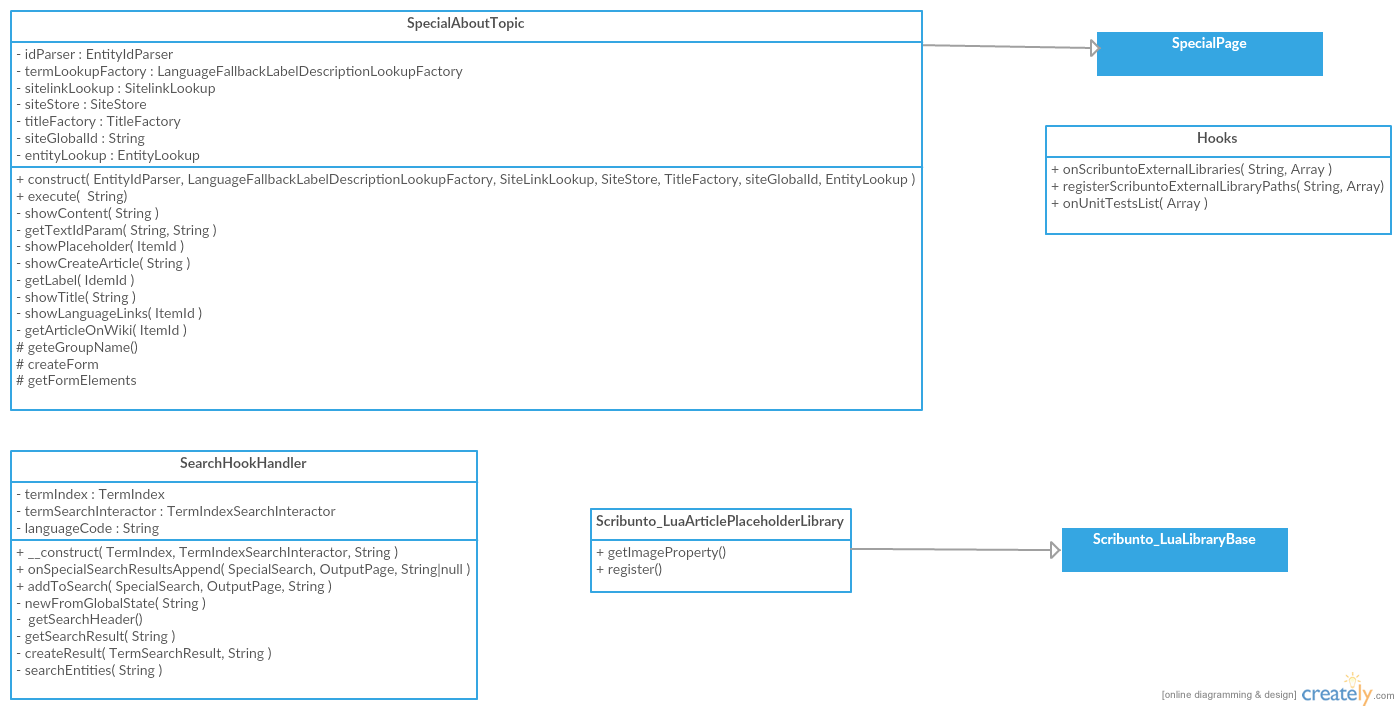
\includegraphics[width=\textwidth]{diagrams/ArticlePlaceholderClassDiagram.png}
	\caption{Class diagram of PHP classes}
	\label{fig:ClassDiagramPHP}
	\end{figure}
	\section{Smart red links}\label{sec:redLinks}
	Red links on Wikipedia display a title of an article, that does not exist yet but is wished by linking to an empty editing page. It is difficult to connect a title to a Wikidata item since the item does not necessarily have the same label as the title of the page. Therefore linking red links to ArticlePlaceholder is rather demanding and not in the scope of this thesis. \\
	However, there is a discussion Discussion page smart red links on how this could be realized, which is summarized in this chapter. \citep{wiki:22} \\
	\\
	The ideal plan is to have \textit{smart red links}, which are connected to a Wikidata item. In order for this to work, the Wikidata sitelinks could be used. Basically there would be \textit{virtual sitelinks}, so editors could connect links to non-existing articles on Wikidata the same way links to existing articles would be added. This way, the text of the article and its Wikitext would not change. On Wikidata, those links could either be in an own section or be displayed in red. \\
	There are multiple ways for editors to add those sitelinks to Wikidata. Existing red links would have to be migrated by editors. Clicking a red link that is not yet connected could lead the editors to a page asking them for the same article in another language and then automatically add the red link to the corresponding Wikidata item. If none exists there is still the possibility to just add the Wikidata item ID. \\
	If an editor adds a red link, they could be asked to add it to the corresponding Wikidata item before saving their edit. \\
	In the case of an editor using ContentTranslation, the link would be added automatically since the article in another language is known. \\
	\\
	As this would also give editors an overview over wanted pages in Wikidata, there are more benefits than only having ArticlePlaceholder connected to red links such as being able to find translatable articles easily.
	\section{Setting up the extension}
	To enable and configure an extension in MediaWiki, the extension needs to have a file called \texttt{\justify ExtensionName.php}, which in this case would be \texttt{\justify ArticlePlaceholder.php}. \texttt{\justify ArticlePlaceholder.php} contains declarations and definitions important to this extension. \\
	To register the extension in MediaWiki, in the file \texttt{\justify LocalSettings.php} the ArticlePlaceholder is included with \texttt{\justify require\_once ``\$IP/extensions/ArticlePlaceholder/ArticlePlaceholder.php'';}. \\
	Additionally the extension uses the global variable \texttt{\justify \$wgArticlePlaceholderImageProperty}. This is needed for the user installing the extension to specify the image property of their repository. In the case of Wikidata this would be \textit{``image'' (P18)}. \citep{wiki:23}
	\section{SpecialPage}

The SpecialPage \texttt{\justify Special:AboutTopic} uses multiple services provided by either Wikibase or MediaWiki. It also extends the class \texttt{\justify SpecialPage} provided by MediaWiki. The class is called \texttt{\justify SpecialAboutTopic} and can be found in the namespace \texttt{\justify ArticlePlaceholder\textbackslash{}Specials}. \\
The SpecialPage serves two purposes: It creates the form for the SpecialPage itself and is used to display the ArticlePlaceholder. \\
From a users perspective there are two ways of passing an entity ID to the extension. 
The one option is to enter the ID on the SpecialPage. The SpecialPage is created by an HTML form in the function \texttt{\justify createForm()}, which adds HTML to the \texttt{\justify OutputPage} object provided by MediaWiki. \\
When the entity ID is passed, there is a check whether this entity actually exists. This is done with the \texttt{\justify EntityLookup} provided by Wikibase. \\ If the entity ID does not exist, the user will get the form again with an additional error message. \\
\\
There is the other option to get to an ArticlePlaceholder to do that directly via the URL, for example in the following way. 
\begin{center}
\colorbox{Gray}{\lstinline[basicstyle=\ttfamily\color{white}]|Special:AboutTopic/Q5279|}
\end{center}

If the entity ID exists, the SpecialPage needs to check whether there is already an article on this Wiki for the item. This is done with the \texttt{\justify SiteLinkLookup} service by Wikibase. The function \texttt{\justify getArticleOnWiki( \$entityId)} is called. In case an article exists, it returns the title of that article. The user is then forwarded to that article with the \texttt{\justify redirect( \$url )} function of the \texttt{\justify OutputPage} class.
The flowchart for the described code can be seen in Figure~\ref{fig:createpl}. 
\begin{figure}[H]
	\centering
	\tikzstyle{block} = [rectangle, draw, 
    text width=5em, text centered, rounded corners, minimum height=4em]
\tikzstyle{error} = [draw, ellipse, node distance=3cm,
    minimum height=2em]
\tikzstyle{line} = [draw, -latex']
\tikzstyle{cloud} = [draw, ellipse, node distance=3cm,
    minimum height=2em]
\tikzstyle{final} = [diamond, draw, 
    text width=4.5em, text badly centered, node distance=3cm, inner sep=0pt]

\sffamily

\begin{tikzpicture}[node distance = 2cm, auto]
    % Place nodes
    \node [block] (execute) {execute};
    \node [block, below of=execute] (showContent){show content};
    \node [block, below of=showContent] (itemIdParam) {getItemId Param};
    \node [cloud, below of=itemIdParam] (entityId) {entityId?};  
    \node [block, below of=entityId] (createForm) {createForm};
    \node [final, right of=createForm] (Html) {HTML};
    \node [cloud, left of=createForm] (hasEntity) {hasEntity?};
    \node [cloud, below of=hasEntity] (onWiki) {articleOnWiki?};
    \node [error, right of=onWiki] (error) {\textcolor{red}{error}};
    \node [final, below of=onWiki] (redirect) {redirect};
    \node [final, right of=redirect] (placeholder) {show Placeholder};
    % \node [final, right of=placeholder] (JS) {JavaScript};
    % Draw edges
    \path [line] (execute) -- (showContent);
    \path [line] (showContent) -- (itemIdParam);
    \path [line] (itemIdParam) -- (entityId);
    % \path [line] (entityId) -- (createForm);
    \path [line] (entityId) -- (createForm) node [midway, above, sloped, -latex'] (textnode) {no};
    \path [line] (createForm) -- (Html);
    \path [line] (entityId) -- (hasEntity) node [midway, above, sloped, -latex'] (textnode) {yes};
    % \path [line] (entityId) -- (hasEntity);
    \path [line] (hasEntity) -- (onWiki) node [midway, above, sloped, -latex'] (textnode) {yes};
    %\path [line] (hasEntity) -- (onWiki);
    \path [line] (hasEntity) -- (error) node [midway, above, sloped, -latex'] (textnode) {no};
    % \path [line] (hasEntity) -- (error);
    \path [line] (error) -- (createForm);
    \path [line] (onWiki) -- (redirect) node [midway, above, sloped, -latex'] (textnode) {yes};
    % \path [line] (onWiki) -- (redirect);
    \path [line] (onWiki) -- (placeholder) node [midway, above, sloped, -latex'] (textnode) {no};
    % \path [line] (onWiki) -- (placeholder);
    % \path [line] (placeholder) -- (JS);
\end{tikzpicture}

\rmfamily
	\caption{Flowchart for creating a placeholder}
	\label{fig:createpl}
\end{figure}

If there is no article for the passed item, an ArticlePlaceholder is created. In order to do this, a template on the Wiki is invoked, which calls the Lua module. Additionally \texttt{\justify OOUI} is enable in order to include the JavaScript module. The label of the item is passed to the JavaScript module \texttt{\justify ext.articleplaceholder.createArticle}. The label is used in PHP to set the title of the page, too. The link to other Wikipedia language versions (language links) are set in PHP. The \textit{sitelinks} are read from the \texttt{\justify SiteStore} service provided by Wikibase. They are assembled from their language code and the page name with a colon in between. For example, the page linking to English Wikipedia article on ``Ada Lovelace'' would be \texttt{\justify en:Ada Lovelace}\\
Showing a placeholder can be described as in the chart in Figure~\ref{fig:showpl}. 
\begin{figure}[H]
	\centering
	\tikzstyle{block} = [rectangle, draw, 
    text width=5em, text centered, rounded corners, minimum height=4em]
\tikzstyle{line} = [draw, -latex']

\sffamily

\begin{tikzpicture}[node distance = 3cm, auto]
    % Place nodes
    \node [block, align=center] (showPl) {show Placeholder};
    \node [block, below of=showPl] (callTemp) {call template};
    \node [block, left=2em of callTemp] (showCA){showCreate Article};
	\node [block, right=2em of callTemp] (showTitle) {showTitle};
	\node [block, right=2em of showTitle] (showLl) {showLang-uagelinks};
	\node[block, below of=showCA] (passL) {pass label};
	\node [block, right=2em of passL] (enableOOUI) {enableOOUI};
	\node [block, below of=passL] (createB) {create Button};
	\node [block, right of=createB] (JS) {JavaScript module};
	\node [block, below of=showLl] (sl) {getSitelinks ForItem};
	\node [block, below of=sl] (lcpn) {Language Code:Page Name};
	
    % Draw edges
    \path [line] (showPl) -- (showCA);
	\path [line] (showPl) -- (callTemp);
	\path [line] (showPl) -- (showTitle);
	\path [line] (showPl) -- (showLl);
	\path [line] (showCA) -- (enableOOUI);
	\path [line] (showCA) -- (passL);
	\path [line] (enableOOUI) -- (createB);
	\path [line] (passL) -- (createB);
	\path [line] (createB) -- (JS);
	\path [line] (showLl) -- (sl);
	\path [line] (sl) -- (lcpn);
\end{tikzpicture}

\rmfamily
	\caption{Flowchart for showing a placeholder}
	\label{fig:showpl}
\end{figure}

	\section{Display}
	The display is one of the main parts of the ArticlePlaceholder as it is user-facing and therefore needed an initial default design. \\
	\begin{figure}[H]
		\centering
		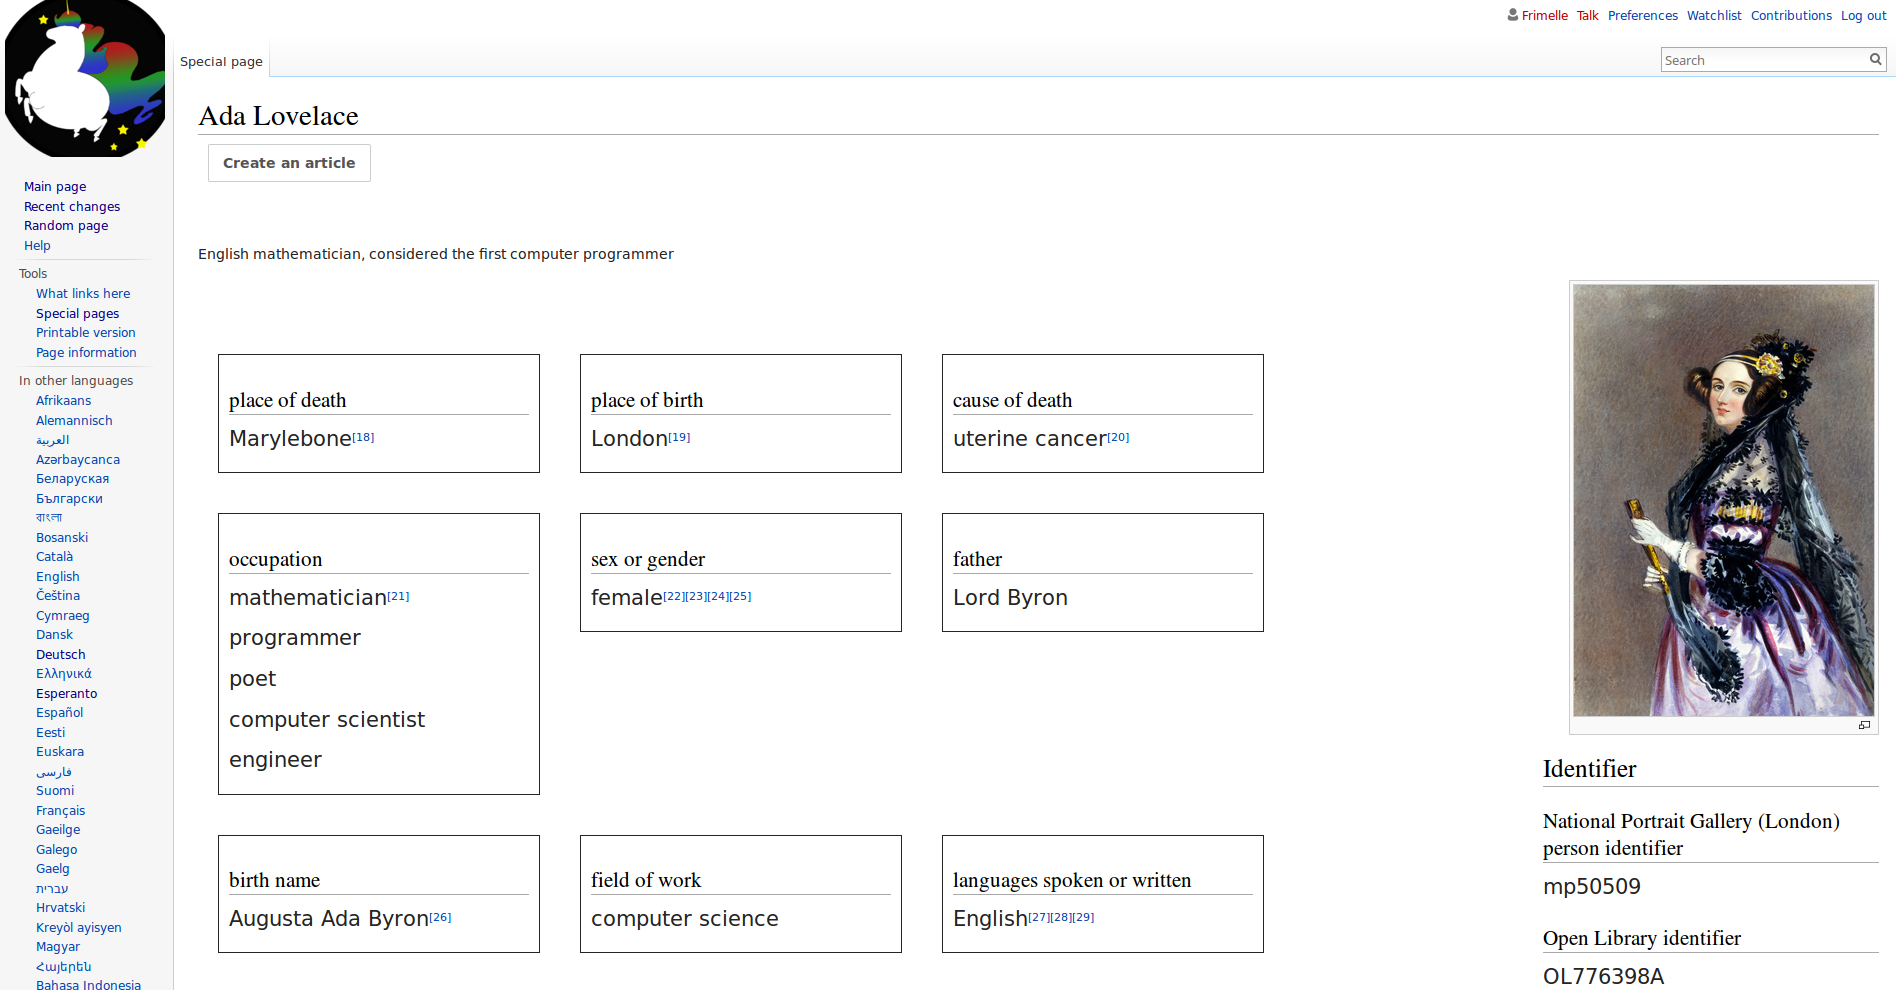
\includegraphics[width=\textwidth]{diagrams/Screenshot-ArticlePlaceholder.png}
		\caption{Screenshot of the ArticlePlaceholder layout as of January 2016}
		\label{screenshot}
	\end{figure}
	The core part of the page are the statement groups. Those consist of a property, one or multiple values, their qualifiers and references. \\
	The statement groups are each in a box with a black border and arranged in a tile layout. The amount of statement boxes per row differs depending on the width of the screen. \\
	The main image of the item is on the right side (for left to right languages) of the page where it would be in articles as well.\\
	The label of the property is the header for each group which is separated from the body by a horizontal line. Multiple values for the same statement are also separated by a line. Their qualifiers are right under the corresponding value. \\
	References can be found in their own section at the bottom of the page sticking to the existing layout of Wikipedia. \\
	The identifier of an item should be in a distinct place in order to be emphasized and distinguishable from the other statements at the same time. They are listed below the main image of the article to the right of the statement groups.
	
	\subsection{Renderer}

Every part of an entity, or item in the case of the ArticlePlaceholder, needs a \textit{renderer} to be displayed. The renderer are written in Lua. They pull data from Wikidata and render it to HTML. They set CSS classes for the HTML elements in order to style them with the CSS module \texttt{\justify ext.articleplaceholder.defaultDisplay.css}. The HTML output of the module is displayed on the \texttt{\justify Special:AboutTopic} ArticlePlaceholder. \\
The MediaWiki conventions for naming Lua modules is 
\begin{center}
\texttt{\justify mw.ext.extensionName.moduleName} 
\end{center}
In order to match them, the default renderer for ArticlePlaceholders is called 
\begin{center}
\texttt{\justify mw.ext.articlePlacholder.entityRenderer}
\end{center}
The entity renderer has getter and setter functions for individual renderers. Therefore every part of the display logic can be overwritten locally on Wikipedia. \\
The Lua module on the Wikipedia is at \texttt{\justify Module:AboutTopic}, which is invoked by \texttt{\justify Template:AboutTopic}. On the entity renderer instance obtained a user with the appropriate rights can call the getter and setter functions. \\
The renderer are as interchangeable as possible so that for example the \texttt{\justify snaksRenderer} can be used by the \texttt{\justify refererenceRenderer} as well as the \texttt{\justify qualifierRenderer}. The scopes of the renderer are therefore limited to their functionality. \\
Wikibase provides a Scribunto interface with functions to access the repository. Wherever possible, the functions provided by this interface were used. This way, the description renderer for example simply wraps \texttt{\justify mw.wikibase.description}. The \texttt{\justify descriptionRenderer} of the ArticlePlacheolder's EntityRenderer is still needed as a seperate service since there must be a possibility for the user to overwrite the renderer. Additionally a CSS class is wrapped around the result of Wikibase's description renderer in order to style it properly. \\
The EntityRenderer module itself takes the entity Id of an item an ArticlePlaceholder is created for. The Lua table for an entity is loaded in the \texttt{\justify renderEntity} function. This table represents the whole entity with all its respective data. Therefore it is performance-wise a very expensive operation. \\

\begin{figure}[H]
	\centering
	\includegraphics[width=\textwidth]{diagrams/EntityRendererMethods.png}
	\caption{Diagram of all renderer functions}
	\label{fig:renderer}
\end{figure}
	\documentclass[11pt]{article}

\usepackage[dvipsnames]{xcolor}
\usepackage{hyperref}
\usepackage{todonotes}
\usepackage{listings}

\title {{Functional requirements}}
\author {Lucie-Aim\'{e}e Kaffee}
\date{}

\begin{document}

\section{Identifier}

To get a list of all external identifier in Wikidata, the item Q19847637, "Wikidata property representing a unique identifier", was used. To get all the Items, that were an instance of (property P31) this item, I used  \href{https://query.wikidata.org}{Wikidata's SPARQL endpoint}. A file with the property Ids is returned. The JSON format was the most useful in this case to be converted to a Lua table. \\

\begin{lstlisting}[frame=single] 
PREFIX wd: <http://www.wikidata.org/entity/>
PREFIX wdt: <http://www.wikidata.org/prop/direct/>

SELECT ?identifier WHERE {
   ?identifier  wdt:P31 wd:Q19847637 . 
}
\end{lstlisting}

\end{document}
	\documentclass[11pt]{article}

\usepackage[dvipsnames]{xcolor}
\usepackage{hyperref}
\usepackage{todonotes}
\usepackage{listings}
\usepackage{soul}
\usepackage[latin1]{inputenc}
\usepackage{tikz}
\usetikzlibrary{shapes,arrows}

\title {{Implementation}}
\author {Lucie-Aim\'{e}e Kaffee}
\date{}

\begin{document}
Test
\end{document}
	\subsection{Style elemts (CSS)}

In order to style the layout elements, CSS classes were assigned in the Lua module. Their looks as well as the create article button's look are adjusted in \texttt{ext.articleplaceholder.defaultDisplay.css}. The main elements belonging in one part in the layout such as the main image and the identifier, that are in one sidebar, are in one common \texttt{div}. Additionally the identifier are all in one \texttt{div}, the \texttt{sidebar}. \\
To not conflict with other MediaWiki style elements, the CSS classes are prefixed with \texttt{\justify articleplaceholder-}. \\
The \texttt{divs} containing the statement groups have a maximum width, so a maximum of three boxes are in one row. The number of columns differs depend on the amount of statements. When the browser window is smaller, the amount of boxes per row adjusts accordingly. Initially it was planned to adjust them to a tiling layout, but since tiling layout in pure CSS would expect the boxes to be ordered vertically in columns this was not possible. It is important to show the most important information in the first row, otherwise the ordering of statement groups would be pointless. \\
In order to be responsive, the extension makes use of \textit{media queries}. Media queries are a convenient way to add new CSS styles for elements that need to be adjusted for different devices. \citep[43]{mediaquery}\\
In MediaWiki with the \textit{resource loader} \texttt{\justify \$wgResourceModules} media queries can be assigned to CSS modules. This way it is possible to load another CSS module (\texttt{\justify ext.articleplaceholder.defaultDisplaySmall.css}), when the screen size is smaller then 930 pixel. This was mainly added in order to avoid the overlapping of the sidebar with image and identifier, and the statement groups.
	\section{Search}
In order to be able to find results from the placeholder in the MediaWiki search, it was necessary to use the SearchHook provided by MediaWiki.
With the help of the \texttt{TermIndexSearchInteractor} provided by Wikibase all items with labels or aliases matching the given search term are returned. The \texttt{TermIndexSearchInteractor} and its respective tests needed to be moved from Wikibase repository to Wikibase library in order to be accessible for both, client and repository. This was done by the author in a commit to the Wikibase code \footnote{\href{https://gerrit.wikimedia.org/r/\#/c/243723/}{Gerrit link}}.

From those a string containing the label of the item, displayed as a link to the special page with the corresponding entity ID, and the description of the item in case there are multiple results.  \\
If the result is not empty, the results are added to the search page as Wikitext. \\
\todo{filtern der Resultate}
\href{https://www.mediawiki.org/wiki/Manual:Hooks/SpecialSearchResultsAppend}{Manual:SpecialSearchResultsAppend}
	\section{Ordering of statement groups}\label{ordering-stat}

To find a technical solution to this problem, there was a "Request for comment" page set up. \citep{wiki:24} \\

The collection of ordered property Ids are stored on one page in the \textit{mediawiki namespace}. This namespace ``is used to hold system messages and other important content''. \citep{wiki:17} It can only be edited by administrators. This page is called \texttt{\justify MediaWiki:Wikibase-SortedProperties}. Since the page name is set in the code, it is a constant variable. \\
The code for the ordering is not merged yet since it was decided to make it part of the Wikibase code instead of only being in the extension. That offers the possibility to reuse the code without having to build up a dependency from Wikibase to the ArticlePlaceholder extension. \\
\\
For now, the page needs to exist on the local Wikipedia. If that's not the case, or if the page is empty or filled with non-text content, the corresponding exception is thrown. For that purpose an \texttt{\justify ArticlePlaceholderException} was created, which extends PHP's \texttt{\justify RuntimeException} to add a message specific to the extension.\\
In the class \texttt{\justify PropertyOrderProvider} the page is parsed to a PHP Array. In this Array, the property Ids are the keys and the ordinal numbers the values. \\

To get the content of the content of the page, the MediaWiki function \texttt{\justify getNativeData()} is used. This page content is parsed in the function \texttt{\justify parseList( \$pageContent )}. To remove all comments in the HTML multiple line comment style, the following regular expression is used.
\begin{lstlisting}[frame=single]
@<!--.*?-->@s
\end{lstlisting}
The \texttt{\justify @} is the delimiter. All comments matching this pattern are replaced with empty Strings. \\
After removing all comments, all Strings matching the following regular expression are written into an Array.
\begin{lstlisting}[frame=single] 
@^\*\s*([Pp]\d+)@m
\end{lstlisting}
This regular expression matches all Strings, that contain an asterisk, optional whitespace, and a upper or lower case \textit{P} followed by a number.
The Array is flipped, to have the properties as keys. This is important when it comes to using the Array in Lua. It is not used in the \texttt{\justify mw.ext.articlePlaceholder.entityRenderer.lua} module yet, but will be in the future. It will be called similar to the image property ID. Then as it is done now with the property IDs in the case of the identifiers, every property ID contained in an item can be compared and ordered accordingly to the ordinal number of the Array. \todo{better explanation} After the sorting is implemented, it is very easy to limit the number of statements, since less important statements can be identified accordingly to their ordinal number. \\
An instance of the class is created in the \texttt{\justify ArticlePlaceholderServices}. \\
In the class \texttt{\justify Scribunto\_LuaArticlePlaceholderLibrary} in the \texttt{\justify ArticlePlaceholder\textbackslash{}Lua} namespace with the help of \texttt{\justify ArticlePlaceholderServices} the Array with the property order is returned in the function \texttt{\justify getPropertyOrder}, which then can be called in the Lua module. This is explained in more detail in the Chapter \ref{including-lua}: \nameref{including-lua}.

	\section{Including Lua}\label{including-lua}

\todo[inline]{The whole text}
	\section{Internationalization}

The extension includes an \texttt{\justify i18n} folder in order to be able to localize all strings needed by the extension. This is the way predefined by MediaWiki.  Every message needed by the extension has a unique message key. This keys are mapped to the text in the different languages. The key-value pairs are stored as JSON. \citep{wiki:34} \\
The keys need to be unique not only in the ArticlePlaceholder extension but also must not conflict with MediaWiki's and its other extensions' keys. Therefore they start with \texttt{\justify articleplaceholder-}. Due to MediaWiki conventions, they are all lower case and may not contain spaces. \\
The documentation for every message is stored in the \texttt{\justify qqq.json} file. The other messages are in the JSON files with the appropriate language key. While developing, it is only necessary to define the English and documentation messages, since the other messages are translated by the community on \url{translatewiki.net}.  \citet{wiki:26} states
\begin{quote}
 \url{translatewiki.net} is a web-based translation platform, powered by the Translate extension for MediaWiki [...] [It has] 6000 translators for over 50[,000] pages from over [twenty] projects including MediaWiki, OpenStreetMap, Mifos, Encyclopedia of Life and MantisBT.
\end{quote}

To load the messages, their directory is added to \texttt{\justify \$wgMessagesDirs}. \texttt{\justify \$wgMessagesDirs} is an associative array that maps the extension name to the appropriate message directory for the MediaWiki software to extract the messages and their keys. \\
The messages can now be used in PHP, JavaScript and Lua with their respective methods provided by MediaWiki. In PHP the message can be loaded using the function \texttt{\justify wfMessage} with the message key as a parameter. The syntax for Lua is \texttt{\justify mw.message.new( message-key ):plain()} and for JavaScript \texttt{\justify mw.message( message-key ).escaped()}. Due to the similar syntax of Lua and JavaScript, the call to the function is similar too. \\ 
In the last two examples, the messages are additionally escaped.
	\section{Unit tests}

MediaWiki, and therefore Wikibase too, use \textit{PHPUnit} for automated testing. PHPUnit is a test framework for PHP. \\
The tests for each class are named according to the class names with the suffix \textit{Test}. \\
\begin{quote}
 ``When we are writing a test in which we cannot (or choose not to) use a real depended-on component (DOC), we can replace it with a \textit{Test Double}. The \textit{Test Double} doesn't have to behave exactly like the real DOC; it merely has to provide the same API as the real one so that the SUT [system under test] \textit{thinks} it is the real one'' states \citet{testing}. 
\end{quote}
PHPUnit provides the option to create so called \textit{mocks} as test doubles. In the test class \texttt{SearchHookHandlerTest}, for example, the SpecialPage \texttt{SpecialSearch} is mocked to work on a test double. \\
PHPUnit allows using data providers. Those data providers return an array of arrays, which provide data for a test method. This way, one method can test several different cases with multiple datasets. The arrays can contain a message explaining what the test is about, a parameter passed to the tested method, and the expected value returned. \\
Each test method can contain one or more assertion. Those are able to test whether the result of the tested function equals the expected value. 


	\section{Deployment}

Adding new components to a software needs, according to \citet{deployment}, 
\begin{quote}
	release, installation, activation, deactivation, update, and removal of components. These activities constitute a large and complex process that we refer to as software deployment.  
\end{quote}

To deploy the ArticlePlaceholder extension to Wikipedia, coordination with Wikimedia staff and volunteers was needed. \\
In Wikimedia, people with appropriate rights, volunteers and staff, can deploy. They have a schedule, which can be adjusted to an extension author's needs. Because the author does not have deployment rights on the Wikimedia cluster, cooperation with Wikimedia staff was necessary in order to do the steps described in Figure~\ref{fig:deployTimeline}, which describes the deployment process. \\
\begin{sidewaysfigure}
	\todo[inline]{look into this more!}
	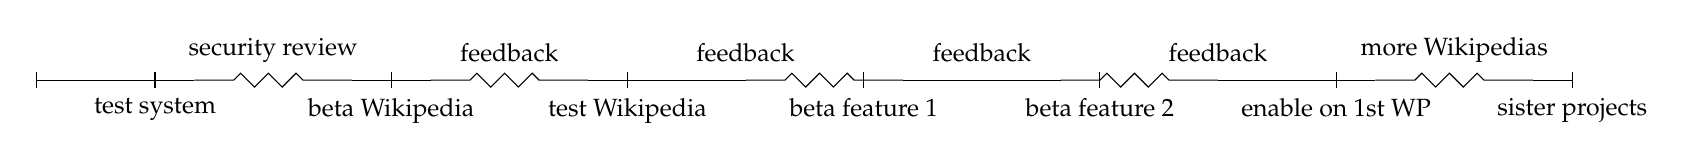
\begin{tikzpicture}[snake=zigzag, line before snake = 5mm, line after snake = 5mm]
		% draw horizontal line   
		\draw (0,0) -- (2,0);
		\draw[snake] (2,0) -- (4,0);
		\draw (4,0) -- (5,0);
		\draw[snake] (5,0) -- (7,0);
		\draw (7,0) -- (9,0);
		\draw[snake] (9,0) -- (11,0);
		\draw (11,0) -- (13,0);
		\draw[snake] (13,0) -- (15,0);
		\draw (15,0) -- (17,0);
		\draw[snake] (17,0) -- (19,0);
		\draw (19,0) -- (19.5,0);
		

		% draw vertical lines
		\foreach \x in {0,1.5,4.5,7.5,10.5,13.5,16.5,19.5}
			\draw (\x cm,3pt) -- (\x cm,-3pt);

		% draw nodes
		\draw (0,0) node[below=3pt] {} node[above=3pt] {$   $};
		\draw (1.5,0) node[below=3pt] {\small test system} node[above=3pt] {};
		\draw (3,0) node[below=3pt] {} node[above=3pt] {\small security review};
		\draw (4.5,0) node[below=3pt] {\small beta Wikipedia} node[above=3pt] {};
		\draw (6,0) node[below=3pt] {} node[above=3pt] {\small feedback};
		\draw (7.5,0) node[below=3pt] {\small test Wikipedia} node[above=3pt] {};
		\draw (9,0) node[below=3pt] {} node[above=3pt] {\small feedback};
		\draw (10.5,0) node[below=3pt] {\small beta feature 1} node[above=3pt] {};
		\draw (12,0) node[below=3pt] {} node[above=3pt] {\small feedback};
		\draw (13.5,0) node[below=3pt] {\small beta feature 2} node[above=3pt] {};
		\draw (15,0) node[below=3pt] {} node[above=3pt] {\small feedback};
		\draw (16.5,0) node[below=3pt] {\small enable on 1st WP} node[above=3pt] {};
		\draw (18,0) node[below=3pt] {} node[above=3pt] {\small more Wikipedias};
		\draw (19.5,0) node[below=3pt] {\small sister projects} node[above=3pt] {};
	\end{tikzpicture}
    \caption{Time line of ArticlePlaceholder deployment}
    \label{fig:deployTimeline}
\end{sidewaysfigure}

\paragraph{Test system}
From the beginning there was a test setup available on Wikimedia Labs\footnote{\url{articleplaceholder.wmflabs.org/mediawiki}}. Wikimedia Labs is 
\begin{quotation}
	the Wikimedia Foundation (WMF)'s cloud computing environment for developing software for the Foundation's operations. It also hosts bots and tools maintained and used by the community to maintain the [F]oundation's projects. 
\end{quotation} \citep{wiki:03}
Besides the bots and scripts running on Wikimedia Labs it is used for various tools and to test software by volunteers as well as WMF's staff.\todo{improve sentence} \\
The test setup was established to give editors as well as the public a first insight into what the extension looks like, what features it offers, and to make them a part of development. It also aims to start a discussion on what can be improved in order for it to be adjusted to the community's needs.

\paragraph{Security review}
To deploy an extension to the Wikimedia cluster, it is necessary to go through a security review by a Security Engineer of the Wikimedia Foundation. \todo{in order to?}
  
\paragraph{Beta Cluster}
The Beta Cluster\footnote{\url{http://en.wikipedia.beta.wmflabs.org/wiki/Main_Page}} is the \textit{WMF integration environment} and used for testing. In order to deploy the extension there, someone with the appropriate deployment rights needed to do code review and then deploy the extension. First issues with a real Wikipedia cluster were identified and adjusted in this step. \\
Meanwhile the communities of all Wikipedias were asked, whether any of them would be interested in being the first Wikipedia to get the extension. Wikipedias interested were asked to open discussion pages to gather the support of the community. (For e-mail send to the \textit{Wikipedia Technical Ambassadors} mailing list, and an extract of the community survey pages see Appendix \ref{})

\paragraph{Test Wikipedia}
Test Wikipedia\footnote{\url{https://test.wikipedia.org/wiki/Main_Page}} is a test setup and \textit{production cluster} by Wikimedia. It is connected to Test Wikidata\footnote{\url{https://test.wikidata.org/wiki/Wikidata:Main_Page}}. From a development perspective, this is the last step of deployment before enabling the extension on a real Wikipedia. This is also another chance to gain more attention and collect input before the Beta feature. Issues can be found and fixed before they break things on a Wikipedia, that is used by a community to do their daily work. \\
\\
These deployment were done in the scope of the thesis. The following steps will need more adjustment, communication, and preparation and therefore are not part of the thesis but will follow in the near future. 

\paragraph{Beta Feature}
Beta Features are experimental functionalities that can be enabled by registered user in their preferences. 
\begin{quotation}
	The primary purpose of Beta Features is to allow for Wikimedia designers and engineers (from the Wikimedia Foundation and community alike) to roll out technical improvements in an environment where large numbers of users can test, give feedback, and use these features in real-world settings.
\end{quotation} \citep{wiki:04}

The next step was to deploy the extension as a beta feature. While having certain requirements for the test set up, the beta feature was supposed to be actually used by the community and therefore needed to fulfill more requirements, building up on what was already archived in the step before. \\
After the first deploy as a beta feature, the feedback by the community needs to be evaluated and the extension needs to be adjusted accordingly. The adjusted beta feature needs not only to consider the feedback again but also to gain the support and trust of the community to be enabled on a Wikipedia by default so all readers can benefit from it.

\paragraph{Deploy to a Wikipedia, enable by default}
To have it actually deployed, the extension must implement the feedback and concerns collected before. Ideally it would be deployed on a Wikipedia, that has a limited amount of articles and editors first, to actually see if it fulfills the needs of the readers it is aiming at and accepted by the existing communities. 

\paragraph{Deploy to more Wikipedias}
It would then be possible and necessary to deploy it to more Wikipedias, that want to participate. 

\paragraph{Deploy to sister projects}
\begin{quote}
\textbf{Wikimedia sister projects} are all the publicly available wikis operated by the Wikimedia Foundation, including Wikipedia. 
\end{quote} \citep{wiki:29}
In the future, it would be great to adjust the extension in a way that it's useful to other Wikimedia projects as well. This is out of the scope for the thesis but something to keep in mind while developing. \\
One of the possible next projects could be Wikivoyage due to its structural similarity to Wikipedia.
\chapter{Conclusion and outlook}

The main goal of this thesis is to increase access to free and open knowledge. Due to the implementation of the ArticlePlaceholder, it is now possible to generate content pages on the Wikipedia for Wikidata data. \\
This is not only a theoretical improvement but also wished by the communities as visible in the discussion pages on the local Wikipedias. (\textit{See Appendix}) \\
In the future, many of the aspects mentioned before will be implemented such as the possibility of content translation, starting the article creation with data from Wikidata, adjusting the extension also for sister projects, and making the ArticlePlaceholder pages indexable. \\
\\
To evaluate how useful the extension is for the different Wikipedias, it will be necessary to observe how many meaningful articles were created and whether they make the need of bot created stubs superfluous. \\
In further research it would be possible to look into natural language processing and creating text from the data displayed. Since this will not necessarily be something the Wikipedia community wishes, it would still be helpful for other use cases of MediaWiki. 

% Include the chapters of the thesis as separate files from the Chapters folder
% Uncomment the lines as you write the chapters

%\include{Chapters/Chapter1}
%\include{Chapters/Chapter2} 
%\include{Chapters/Chapter3}
%\include{Chapters/Chapter4} 
%\include{Chapters/Chapter5} 

%----------------------------------------------------------------------------------------
%	THESIS CONTENT - APPENDICES
%----------------------------------------------------------------------------------------

\appendix % Cue to tell LaTeX that the following "chapters" are Appendices

\chapter{Figures}

\section{Internet Content Languages}

\begin{figure}[H]
	\centering
	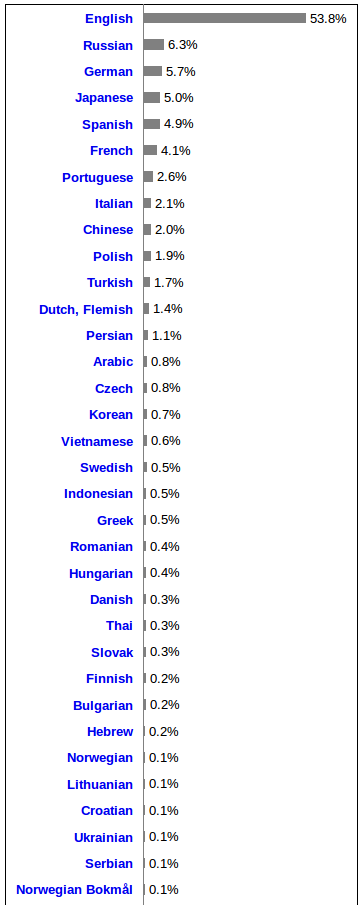
\includegraphics[height=30em]{diagrams/w3techsInternetContentLang.png}
	\caption{Usage of content languages for websites [Screenshot] by \citet{appendixDia:01}}
	\label{fig:w3techLang}
\end{figure}

\section{List of languages by number of native speakers}
\begin{figure}[H]
	\centering
	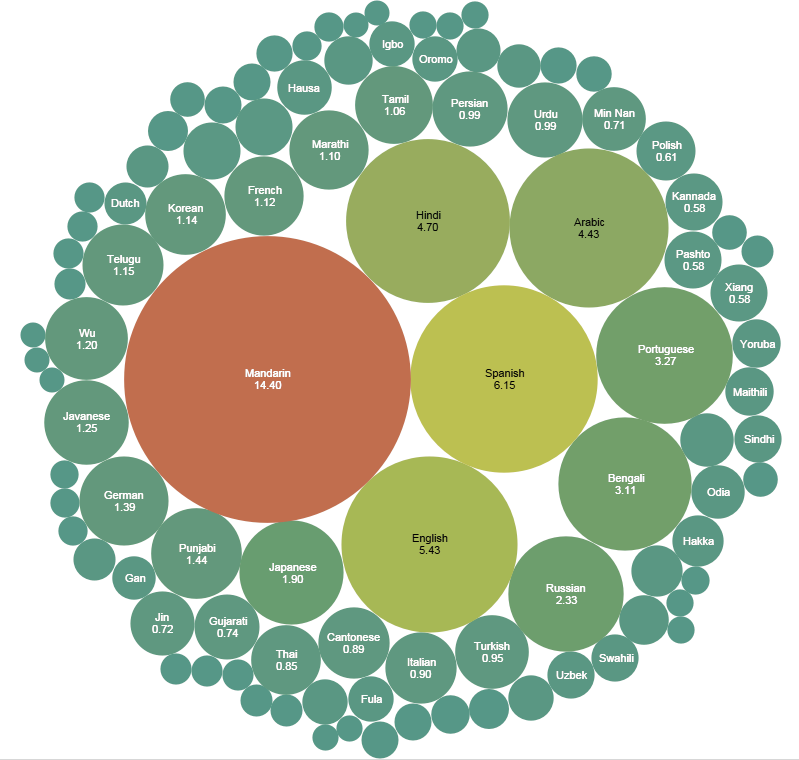
\includegraphics[width=\textwidth]{diagrams/List_of_languages_by_number_of_native_speakers.png}
	\caption{List of languages by number of native speakers by \citet{appendixDia:02}}
	\label{fig:listLang}
\end{figure}

\section{Lists of Wikipedias with over 1.000.000 articles}
\begin{figure}[H]
	\centering
	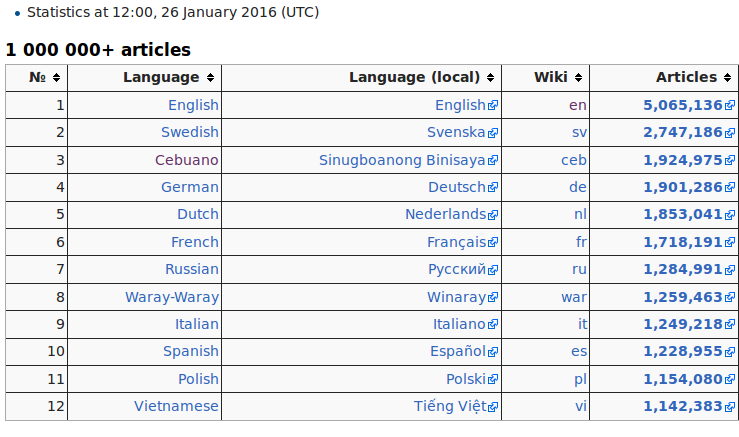
\includegraphics[width=\textwidth]{diagrams/list-of-wikis-articles.png}
	\caption{\citet{appendixDia:03}}
	\label{fig:wikipedias-articles}
\end{figure}

\section{Pageviews Analysis}
\begin{figure}[H]
	\centering
	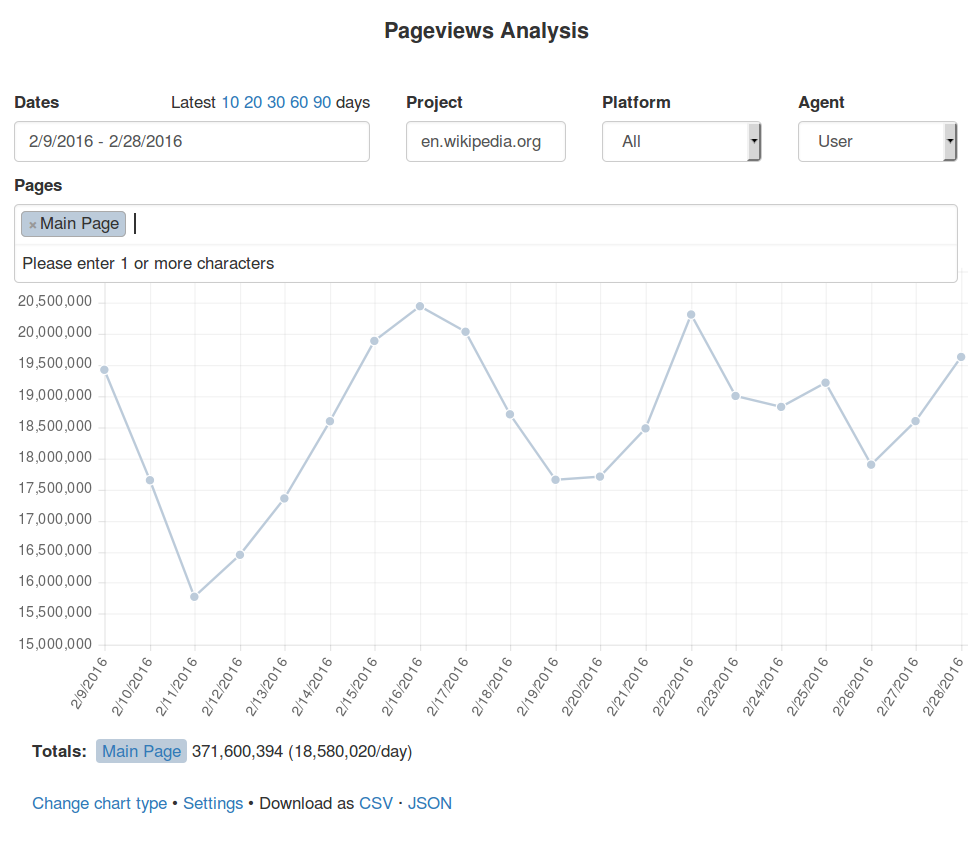
\includegraphics[height=30em]{diagrams/page-views.png}
	\caption{Pageviews Analysis [Screenshot] by \citet{appendixDia:04}}
	\label{fig:pageviews}
\end{figure}
\chapter{Community communication} \label{community}

\paragraph{[Wikitech-ambassadors] Looking for small Wikipedias to test a new feature for them} ~\\
\begin{quote}
As part of my Bachelor’s thesis I worked on an extension called “ArticlePlaceholder” \url{https://www.mediawiki.org/wiki/Extension:ArticlePlaceholder} over the last months. \\
\\
One of the biggest barriers for accessing the knowledge Wikipedia provides is language. \\
\\
There are many topics that are only covered in few, big Wikipedias. People who don’t speak any of these languages don’t have access to all the information available potentially vital to them. \\
\\
The Article Placeholder extensions aims at smaller Wikipedias to support them in increasing access to data available on Wikidata. Article Placeholders are automatically generated content pages in Wikipedia or other mediawiki projects displaying data from Wikidata. They are clearly not actual articles but an overview of data on a topic which does not have an article yet. The design of the page and its content is under the control of the local community via Lua and templates but we will provide defaults so smaller Wikipedias can work with them without having to worry about the technical side of it. \\
\\
I have a test setup on Labs with an example for Ada Lovelace \url{http://articleplaceholder.wmflabs.org/mediawiki/index.php/Special:AboutTopic/Q3} \\
\\
The reader can find these pages by searching for a topic and gets results if there is an Item on Wikidata with the respective label and/or alias. \\
\\
The reader would benefit a lot since even if there is no article on a topic yet, they will still have basic information provided in their language. But it also might increase the numbers of editors due to increased usefulness of that Wikipedia. \\
\\
We are now looking for the first Wikipedias to support the extension by deploying it and giving their input. I am still developing the extension and the first Wikipedias to try it will naturally have a larger say in how it evolves. \\
\\
If your Wikipedia would like to give it a try please let me know. We would start it as a beta feature. \\
\\
Thank you, \\
\\
Lucie (Frimelle)
\end{quote}
\citep{kaffee:01} 

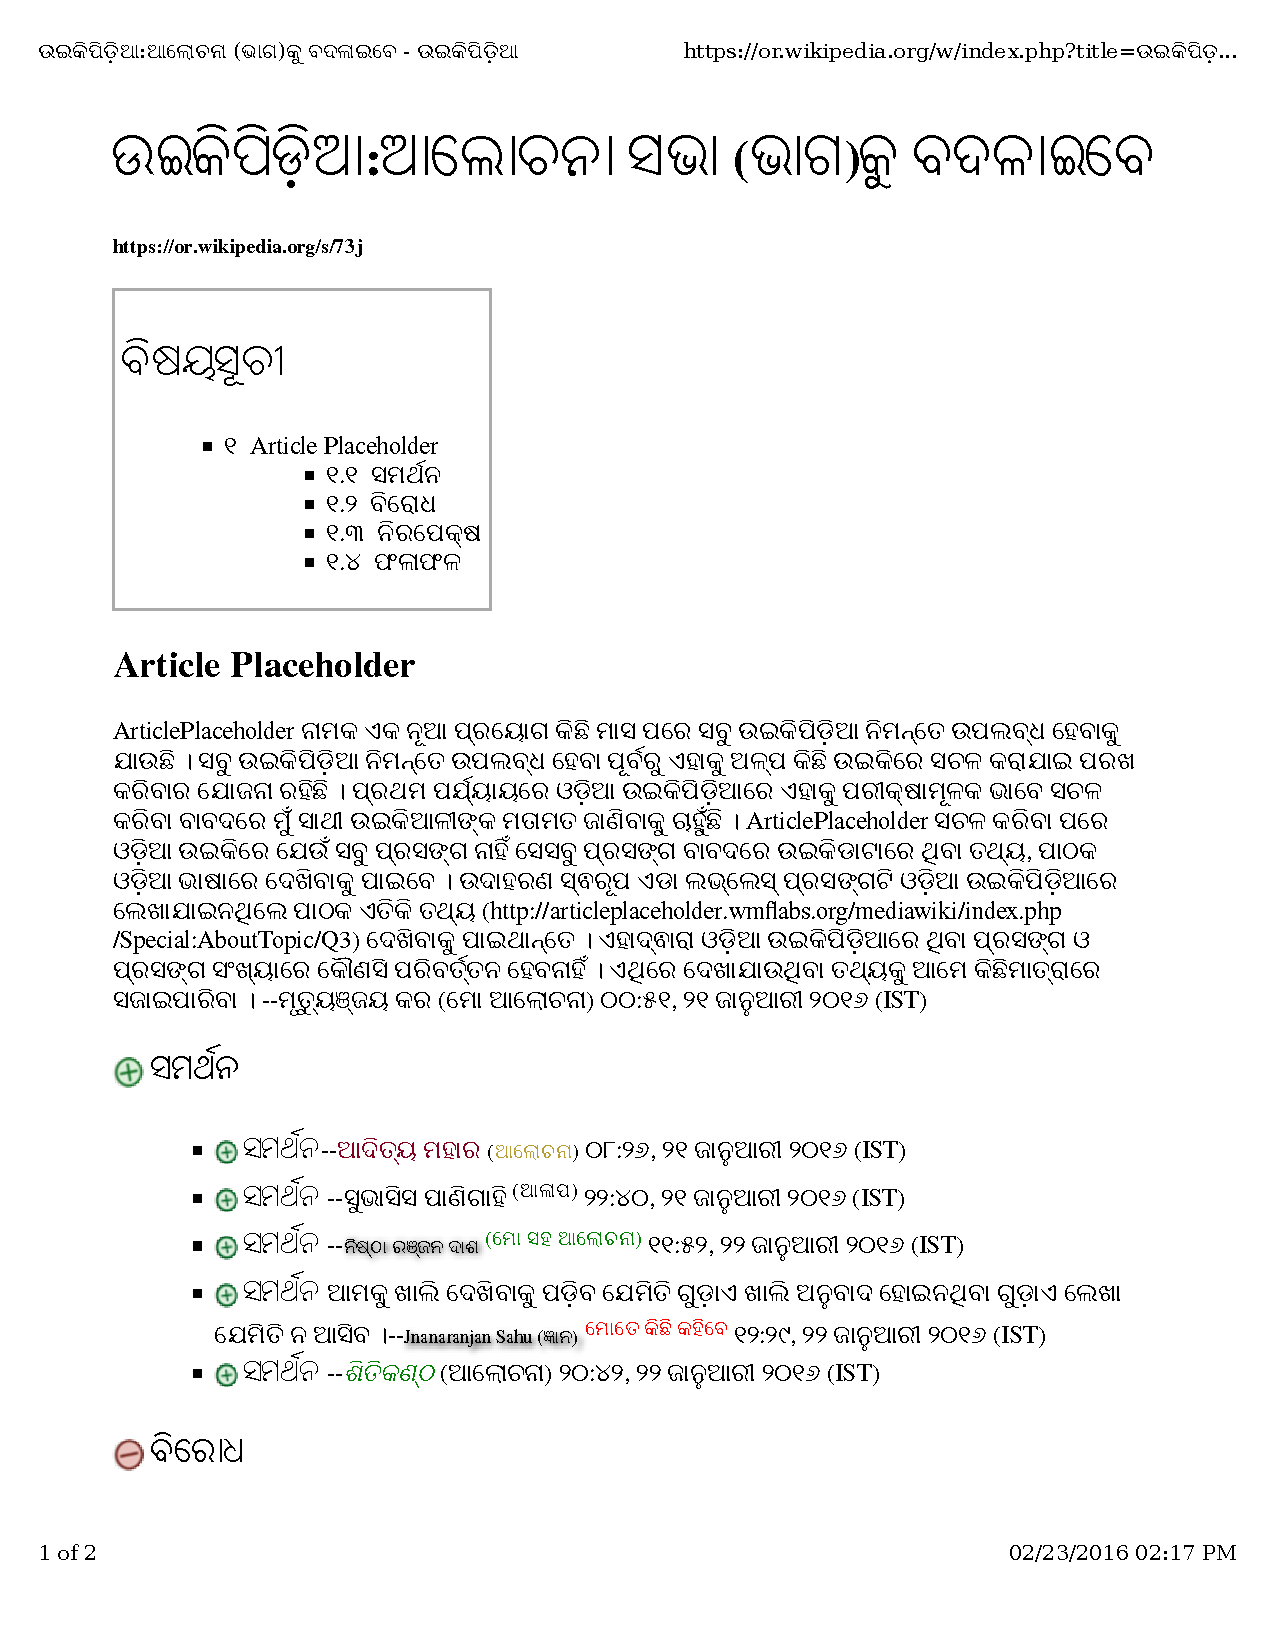
\includepdf[pages=1, scale=0.8, pagecommand={}, link, linkname=odwikipdf]{appendix/odwiki-discussion}
\includepdf[pages=2, scale=0.8, pagecommand={\footnotetext[1]{\cite{wiki:36}}}, link, linkname=odwikipdf]{appendix/odwiki-discussion}

%\hyperlink{odwikipdf.1}{odwikipages}

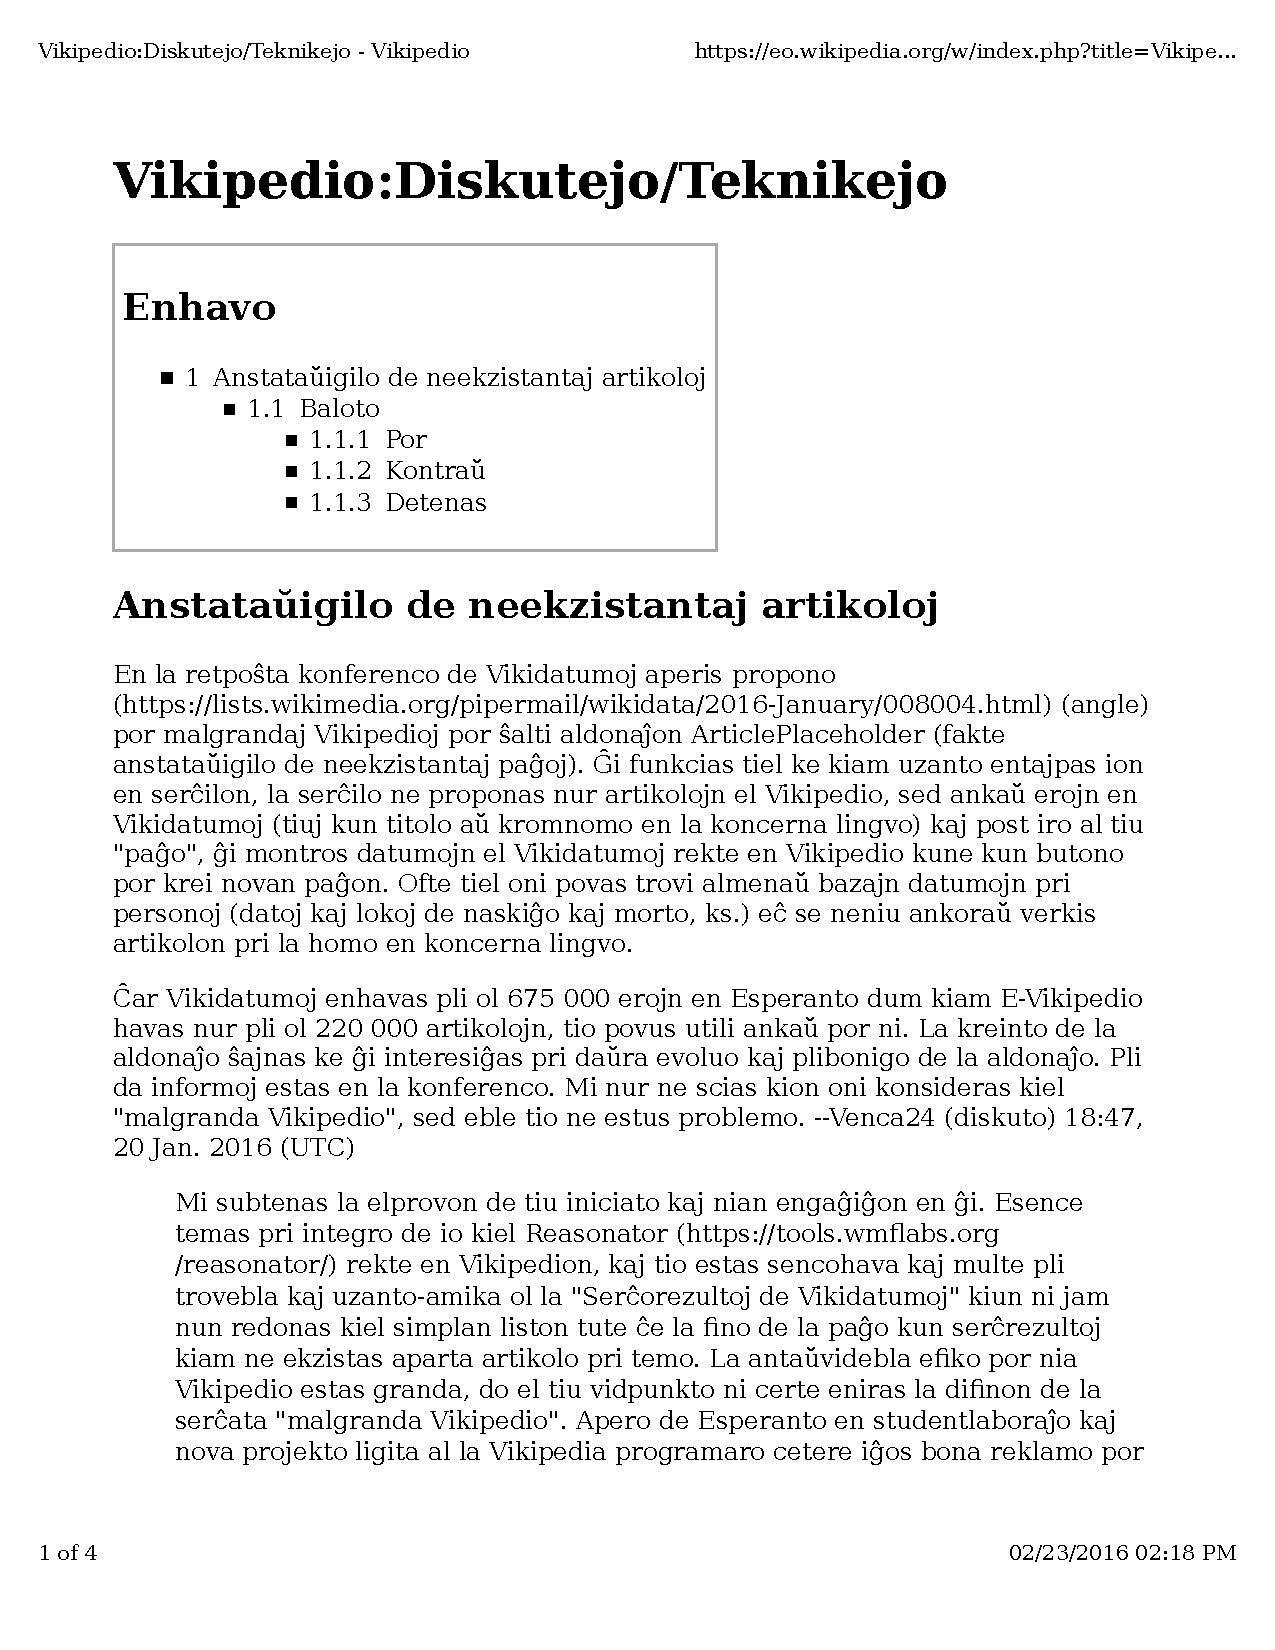
\includepdf[pages=1-3, scale=0.8, pagecommand={}, link, linkname=eowikipdf]{appendix/eowiki-discussion}
\includepdf[pages=4, scale=0.8, pagecommand={\footnotetext[1]{\cite{wiki:35}}}, link, linkname=eswikipdf]{appendix/eowiki-discussion}


\chapter{Code}

% Include the appendices of the thesis as separate files from the Appendices folder
% Uncomment the lines as you write the Appendices

%\include{Appendices/AppendixA}
%\include{Appendices/AppendixB}
%\include{Appendices/AppendixC}

%----------------------------------------------------------------------------------------
%	BIBLIOGRAPHY
%----------------------------------------------------------------------------------------

\printbibliography[heading=bibintoc]

%----------------------------------------------------------------------------------------

\end{document}  
